\section{Modelado conceptual}

\begin{frame}{Introducción}
    \begin{itemize}
        \item Se tiene información y tiempo limitado para pretender modelar el sistema completo.
	    \item Incluso ante suficiente tiempo e información, a menudo un modelo más sencillo (respecto a la complejidad del sistema real) basta para el problema en estudio.
	    \item Al desarrollar un modelo más simple se debe definir el nivel de abstracción al que funcionará.
    \end{itemize}
\end{frame}

\begin{frame}{Definición}
    \begin{itemize}
        \item Un modelo conceptual es una \textit{descripción del modelo de simulación, no específica de un software, que describe los objetivos, entradas, salidas, contenido, supuestos y simplificaciones del modelo}.
        \item Es la abstracción de la parte del sistema que va a representar el modelo de simulación e implica una representación simplificada del sistema real.
    	%\item Es la actividad de decidir qué modelar y qué no modelar.
    \end{itemize}
\end{frame}

\begin{frame}{Requerimientos}
    \begin{itemize}
        \item Un buen modelo conceptual debe:
        \begin{itemize}
        \item Producir resultados precisos para el objetivo propuesto (validez).
        \item Ser creido por los clientes (credibilidad).
        \item Ser factible de construir dentro de las limitaciones de información y de tiempo (factibilidad).
        \item Tener utilidad, es decir, ser fácil de usar, flexible, visual y rápido de ejecutar (usabilidad).
        \end{itemize}
    \end{itemize}
\end{frame}

\begin{frame}{Documentación del modelo conceptual}
    \begin{itemize}
        \item El modelo conceptual no siempre se expresa explícitamente.
	    %\item Es una buena práctica documentar el modelo conceptual y, al hacerlo, proporcionar un medio de comunicación entre todas las partes en un estudio de simulación. 
	    \item Provee un medio de comunicación entre todas las partes involucradas en el estudio de simulación.
    \end{itemize}
    \begin{figure}
        \centering
        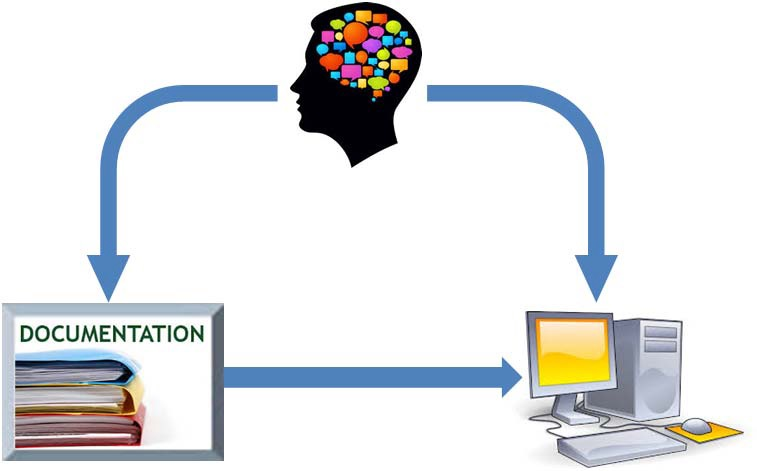
\includegraphics[width=6cm]{images/whereisthemodel.jpg}
        \caption{¿Dónde está el modelo? Tomado de \cite{robinson}}
        %\label{fig:my_label}
    \end{figure}
\end{frame}

\begin{frame}{Documentación del modelo conceptual}
    \begin{itemize}
	    \item No hay estándares establecidos para documentar modelos conceptuales, pero se han propuesto una variedad de enfoques, que incluyen:
	    \begin{enumerate}
	        \item Lista de componentes.
	        \item Diagrama de flujo de procesos.
	        \item Diagrama de actividades.
	        \item Lenguaje unificado de modelado (UML).
	        \item Redes de Petri.
	    \end{enumerate}
    \end{itemize}
\end{frame}